
\begin{frame}
  \frametitle{Improving performance}
  \framesubtitle{Leaf node capacity}

  {\color{white} Show graph of increasing node capacity}

\end{frame}

\begin{frame}
  \frametitle{Improving performance}
  \framesubtitle{Path selection}

  \begin{columns}[T]
    \begin{column}{.4\textwidth}
      \begin{block}{}%
        {\color{white} To minimize pointer dereferences need to optimally %
        traverse nodes in tree}
      \end{block}
    \end{column}
    \begin{column}{.6\textwidth}
      \begin{block}{}
        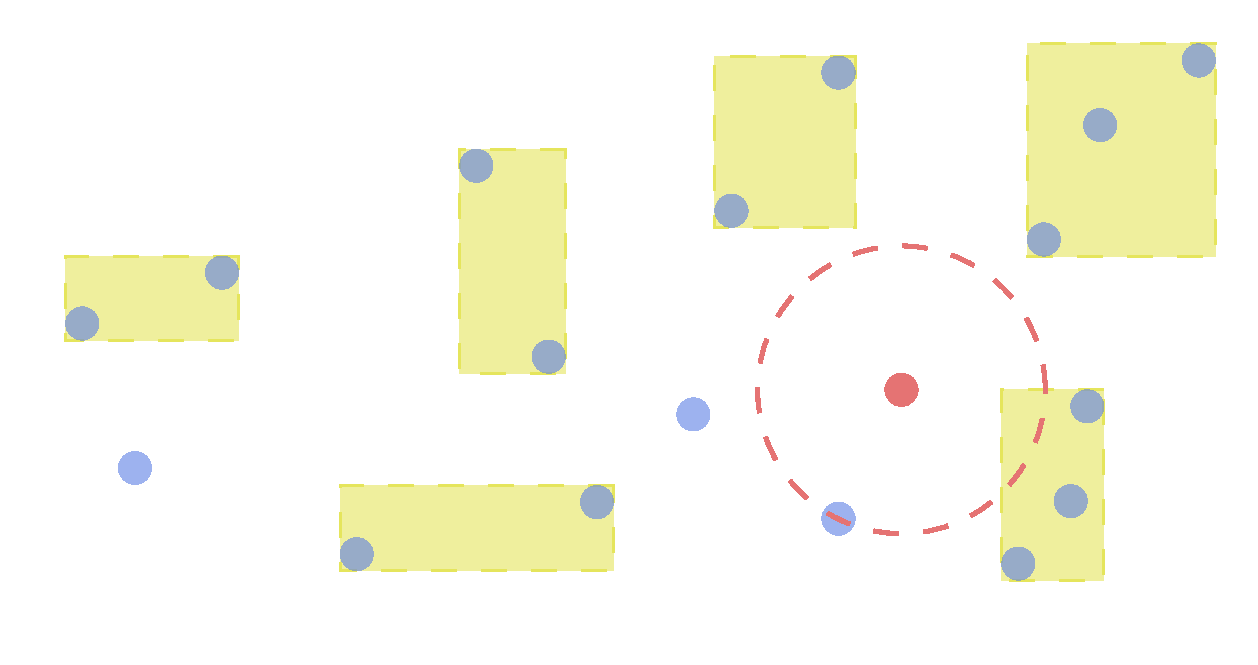
\includegraphics[width=\textwidth]{nn_adjaceny_complex_bound.pdf}
      \end{block}
    \end{column}
  \end{columns}

\end{frame}

\begin{frame}
  \frametitle{Improving performance}
  \framesubtitle{Path selection}

  \begin{figure}
    \centering
    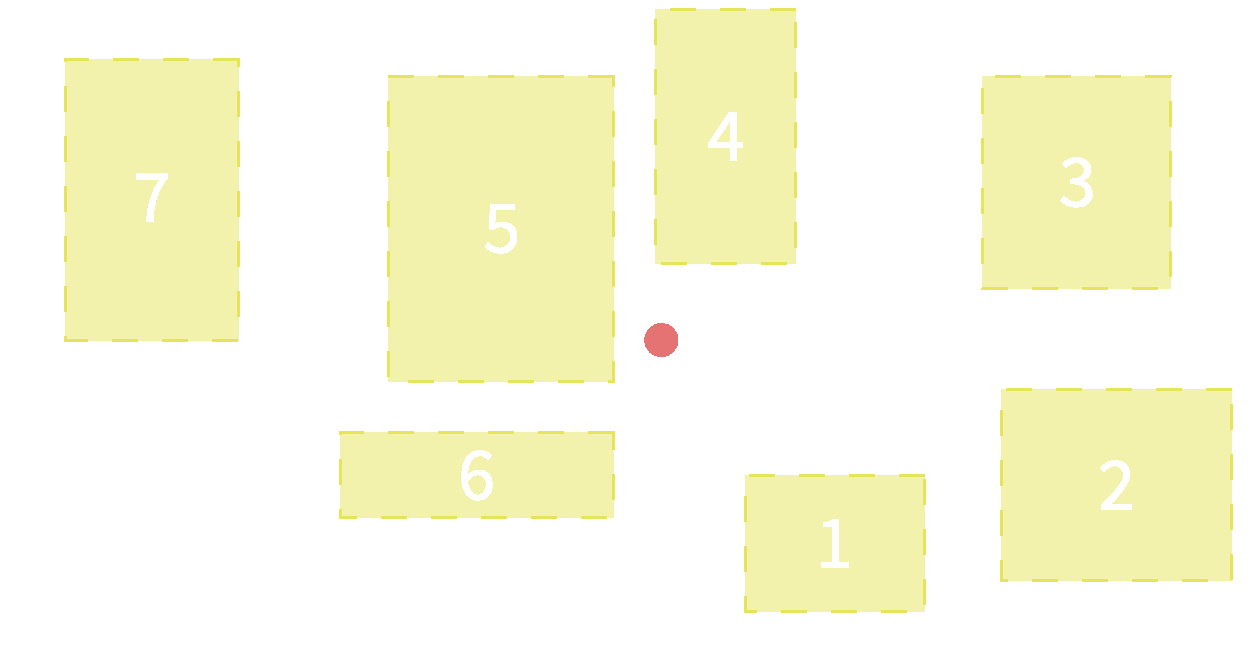
\includegraphics[width=0.85\textwidth]{nn_path_bad.pdf}
  \end{figure}

\end{frame}

\begin{frame}
  \frametitle{Improving performance}
  \framesubtitle{Path selection}

  \begin{figure}
    \centering
    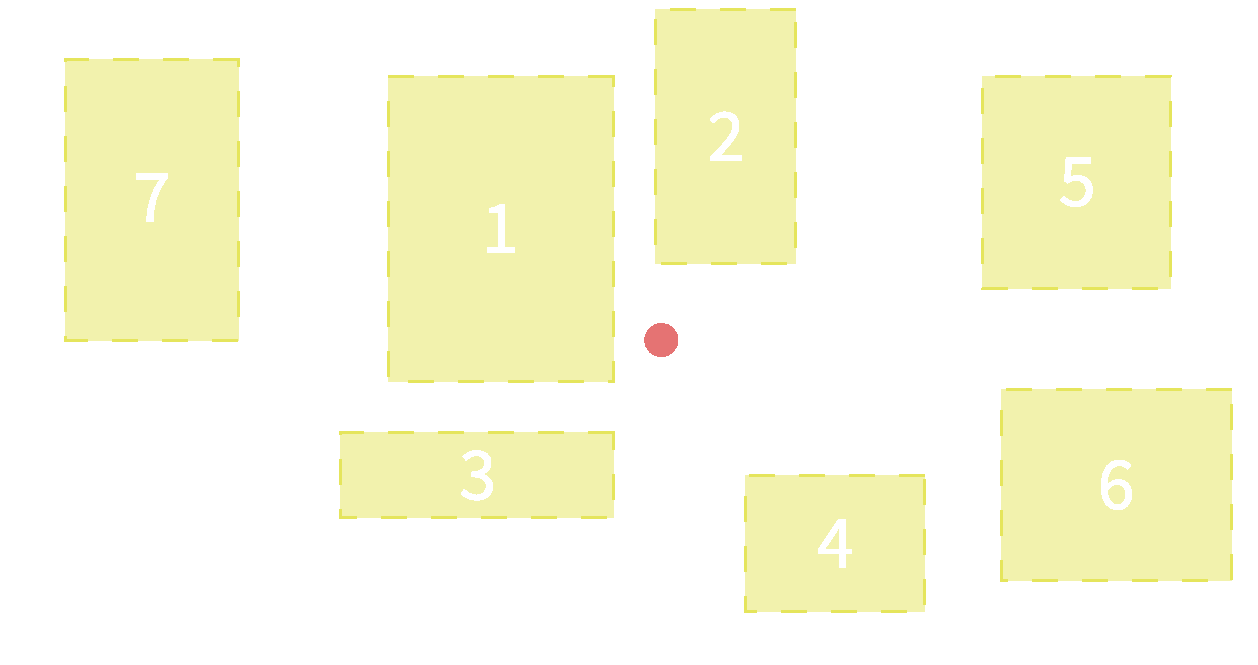
\includegraphics[width=0.85\textwidth]{nn_path_good.pdf}
  \end{figure}

\end{frame}

\begin{frame}
  \frametitle{Improving performance}
  \framesubtitle{Memory management}

  \begin{itemize}
    \item Many modern CPUs have cache line size of 64 bytes
      \begin{itemize}
        \item Size of double is 8 bytes, size of point is 24 bytes
      \end{itemize}
    \item Array of structs memory layout hampers SIMD performance 
  \end{itemize}

\end{frame}

\begin{frame}
  \frametitle{Improving performance}
  \framesubtitle{Memory management}

  \color{white} Show difference in memory organization

\end{frame}
